\documentclass{article}
\usepackage{polski}
\usepackage[utf8]{inputenc}
\usepackage{datetime}
\usepackage{tikz}
\usepackage{graphicx}
\begin{document}
\title{
        {\huge Lekcja 36} \\
        {\large Udowadniamy, że Dziewczyna Leśmiana to ballada filozoficzna}
}
\author{Zbigniew Żołnierowicz}
\date{10.06.2019}
\maketitle
\section{Motyw baśniowości i fantastyki w literaturze. Odwołanie do wskazanego obrazu ``Porwanie królewny'' Witolda Wojtkiewicza i tekstów literackich.}
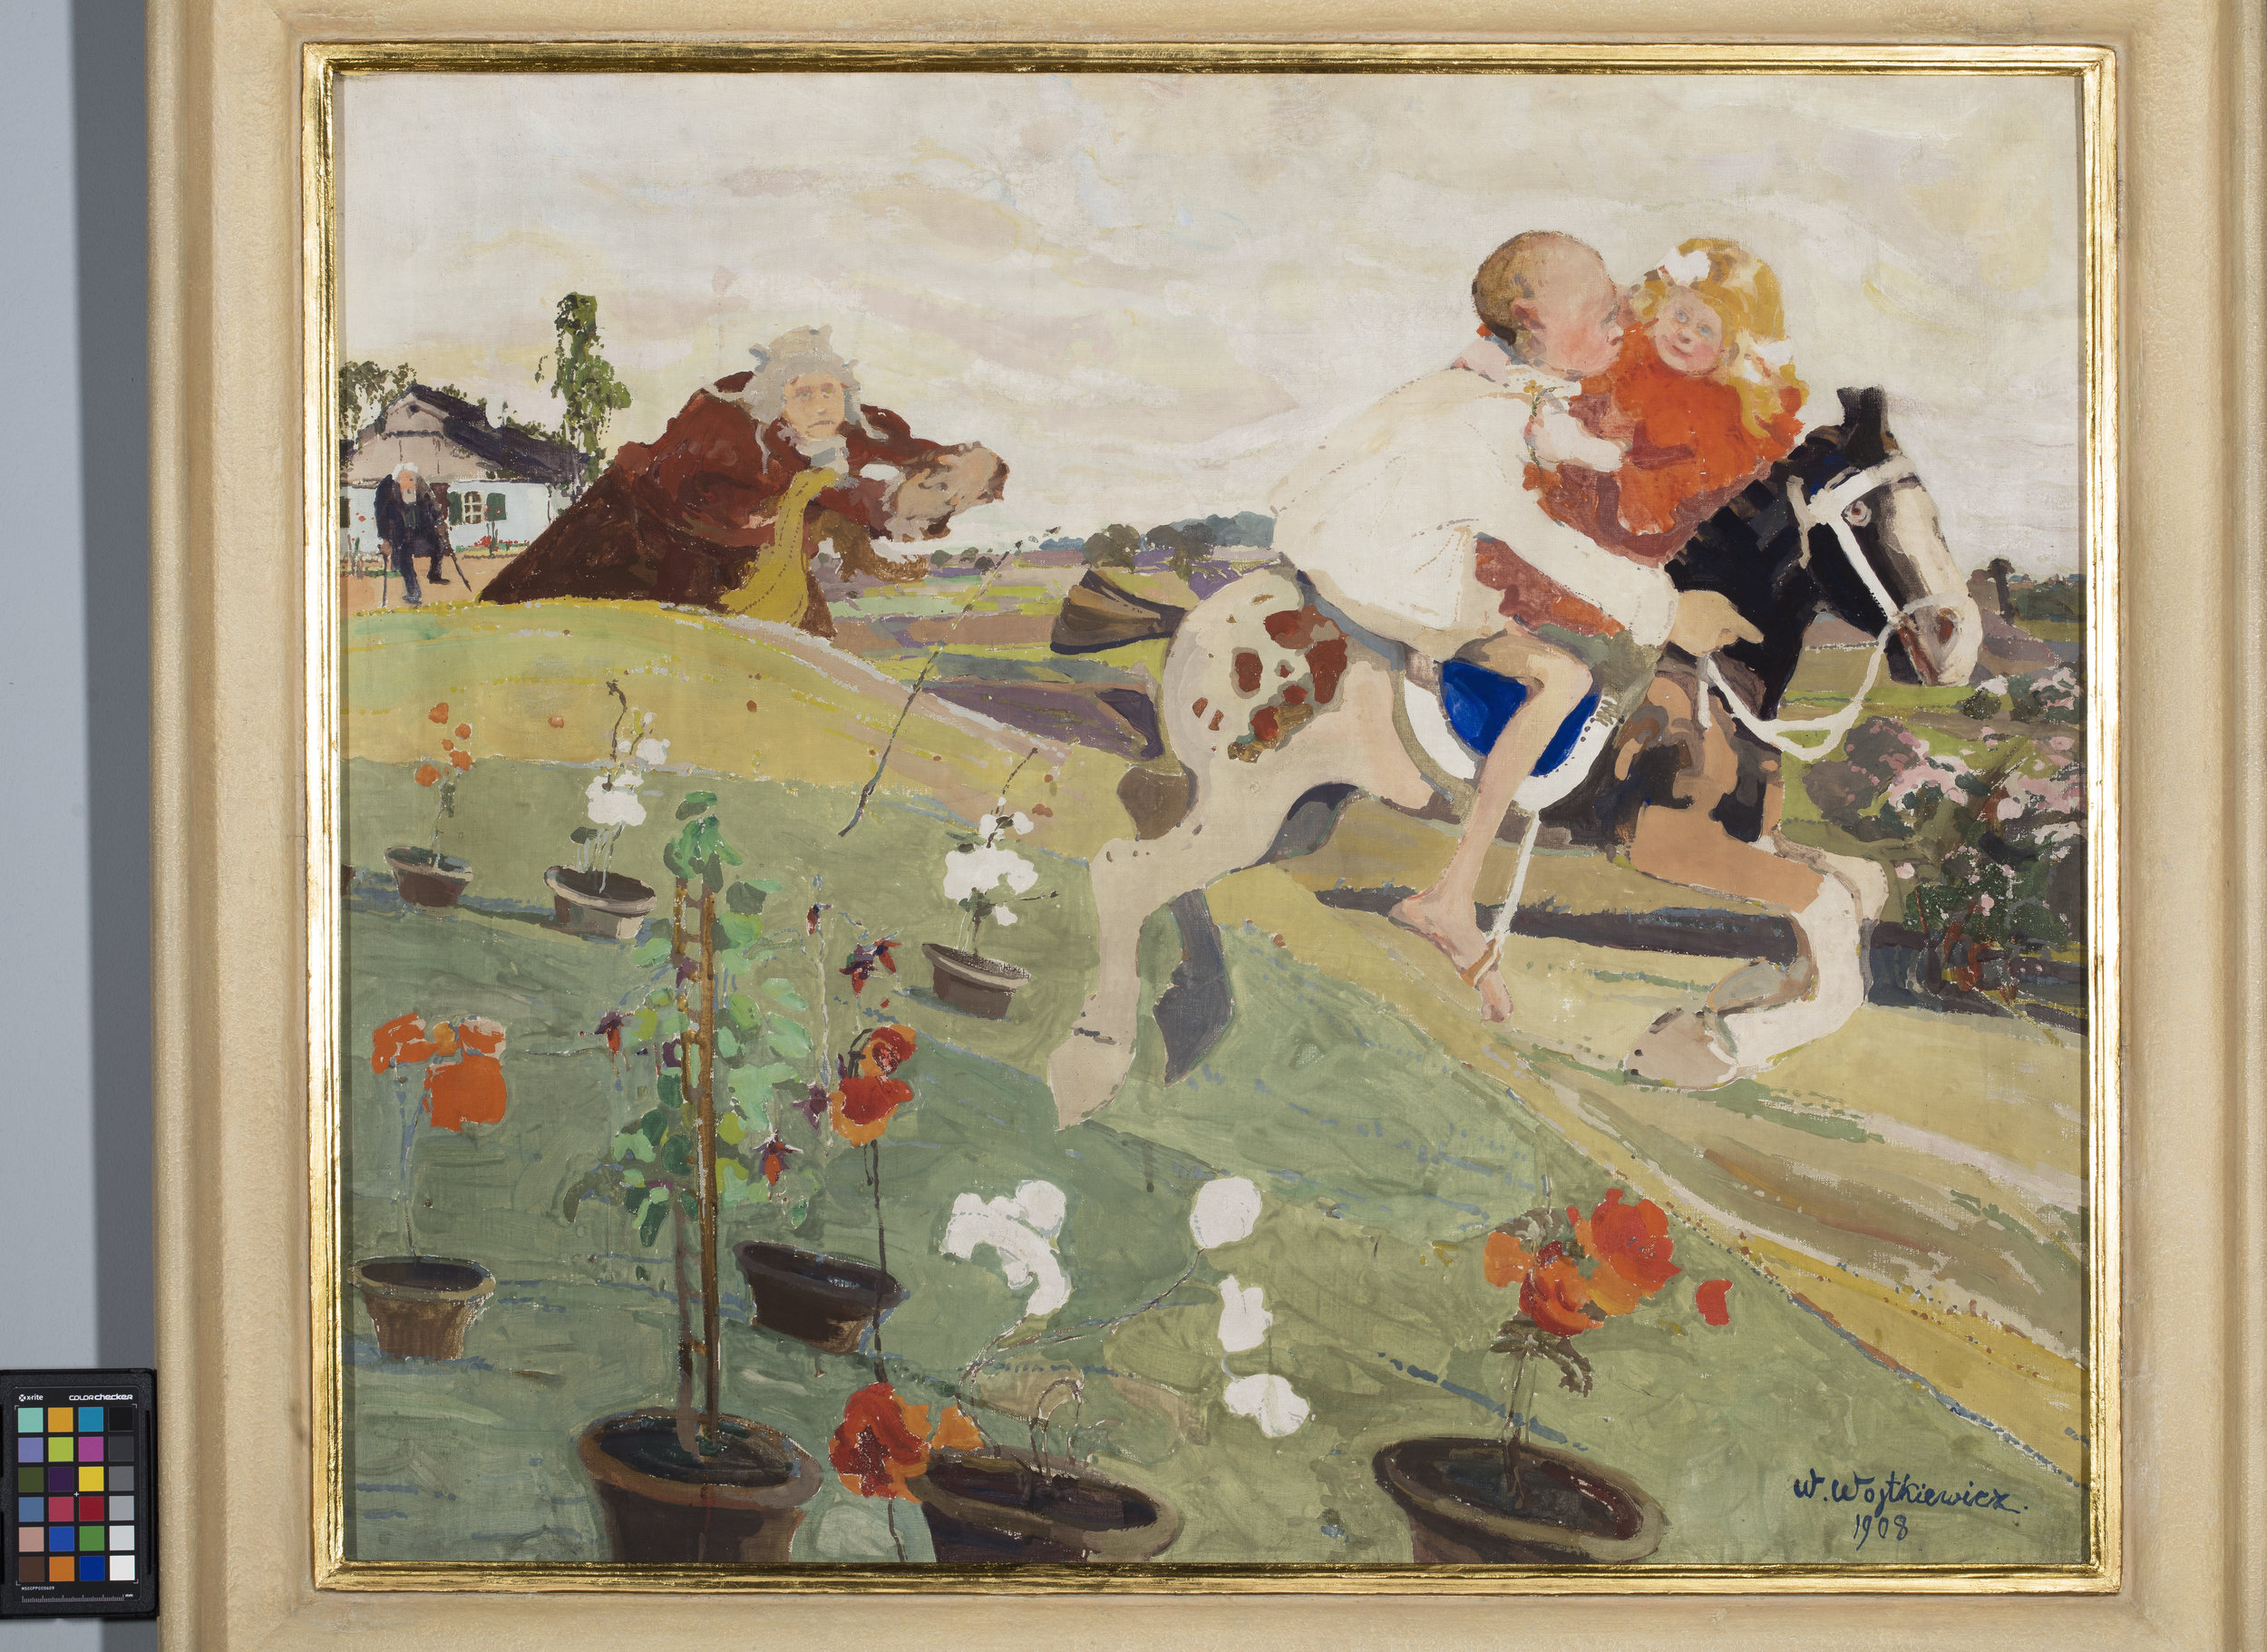
\includegraphics[width=\textwidth]{porwaniekrolewny.jpg}
\end{document}